\documentclass{beamer}
\mode<presentation>
\usepackage{amsmath}
\usepackage{amssymb}
\usepackage{bm}
\usepackage{adjustbox}
\usepackage{subcaption}
\usepackage{enumerate}
\usepackage{multicol}
\usepackage{mathtools}
\usepackage{listings}
\usepackage{url}
\def\UrlBreaks{\do\/\do-}
\usetheme{Boadilla}
\usecolortheme{lily}
\setbeamertemplate{footline}
{
  \leavevmode%
  \hbox{%
  \begin{beamercolorbox}[wd=\paperwidth,ht=2.25ex,dp=1ex,right]{author in head/foot}%
    \insertframenumber{} / \inserttotalframenumber\hspace*{2ex} 
  \end{beamercolorbox}}%
  \vskip0pt%
}
\setbeamertemplate{navigation symbols}{}

\providecommand{\nCr}[2]{\,^{#1}C_{#2}}
\providecommand{\nPr}[2]{\,^{#1}P_{#2}}
\providecommand{\mbf}{\mathbf}
\providecommand{\pr}[1]{\ensuremath{\Pr\left(#1\right)}}
\providecommand{\qfunc}[1]{\ensuremath{Q\left(#1\right)}}
\providecommand{\sbrak}[1]{\ensuremath{{}\left[#1\right]}}
\providecommand{\lsbrak}[1]{\ensuremath{{}\left[#1\right.}}
\providecommand{\rsbrak}[1]{\ensuremath{\left.#1\right]}}
\providecommand{\brak}[1]{\ensuremath{\left(#1\right)}}
\providecommand{\lbrak}[1]{\ensuremath{\left(#1\right.}}
\providecommand{\rbrak}[1]{\ensuremath{\left.#1\right)}}
\providecommand{\cbrak}[1]{\ensuremath{\left\{#1\right\}}}
\providecommand{\lcbrak}[1]{\ensuremath{\left\{#1\right.}}
\providecommand{\rcbrak}[1]{\ensuremath{\left.#1\right\}}}
\providecommand{\rank}{\text{rank}}
\theoremstyle{remark}
\newtheorem{rem}{Remark}
\newcommand{\sgn}{\mathop{\mathrm{sgn}}}
\providecommand{\abs}[1]{\ensuremath{\left\vert #1 \right\vert}}
\providecommand{\res}[1]{\Res\displaylimits_{#1}} 
\providecommand{\norm}[1]{\lVert#1\rVert}
\providecommand{\mtx}[1]{\mathbf{#1}}
\providecommand{\mean}[1]{\overline{#1}}
\providecommand{\fourier}{\overset{\mathcal{F}}{ \rightleftharpoons}}
\providecommand{\system}{\overset{\mathcal{H}}{ \longleftrightarrow}}
\providecommand{\dec}[2]{\ensuremath{\overset{#1}{\underset{#2}{\gtrless}}}}

% this \vec is already defined in your file:
\renewcommand{\vec}[1]{\begin{pmatrix}#1\end{pmatrix}}

\newenvironment{amatrix}[1]{%
  \left(\begin{array}{@{}*{#1}{c}|c@{}}
}{%
  \end{array}\right)
}

\lstset{
frame=single, 
breaklines=true,
columns=fullflexible
}
\usepackage{listings}
\lstset{
  language=Python,
  basicstyle=\ttfamily\small,
  numbers=left,
  numberstyle=\tiny,
  breaklines=true,
  frame=single
}

\title{Matgeo-3.3.3}
\author{AI25BTECH11019-Menavath Sai Sanjana}

\date{}

\begin{document}

\begin{frame}
\titlepage
\end{frame}

\begin{frame}
\frametitle{Question}
Construct an equilateral triangle $\triangle ABC$ with each side $5\,\text{cm}$.  
\end{frame}

\begin{frame}
\frametitle{Solution}
Let
$
\vec{A}=\vec{0\\0},\quad 
\vec{B}=\vec{5\\0},\quad 
\vec{C}=\vec{x\\y}.
$

Using the cosine rule for $\triangle ABC$:
\begin{align}
BC^2 &= AB^2 + AC^2 - 2(AB)(AC)\cos \angle A \quad 
\end{align}

Since $AB=AC=BC=5$:
\begin{align}
25 &= 25 + 25 - 2\cdot25\cos \angle A \quad 
\end{align}

From (2):
\begin{align}
\cos \angle A &= \frac{1}{2}, \quad \angle A = 60^\circ \quad 
\end{align}

Coordinates of $C$:
\begin{align}
\vec{C} = \vec{5\cos60^\circ\\5\sin60^\circ}
= \vec{\frac{5}{2}\\\frac{5\sqrt{3}}{2}}\quad 
\end{align}
\end{frame}


\begin{frame}
\frametitle{Conclusion}
\noindent\textbf{Conclusion:}  
The equilateral triangle $\triangle ABC$ with side $5\,\text{cm}$  
has vertices
$
\vec{A}=\vec{0\\0},\quad 
\vec{B}=\vec{5\\0},\quad 
\vec{C}=\vec{\frac{5}{2}\\\frac{5\sqrt{3}}{2}}.
$
\end{frame}

\begin{frame}
\frametitle{Graphical Representation}

\begin{figure}[ht!]
    \centering
    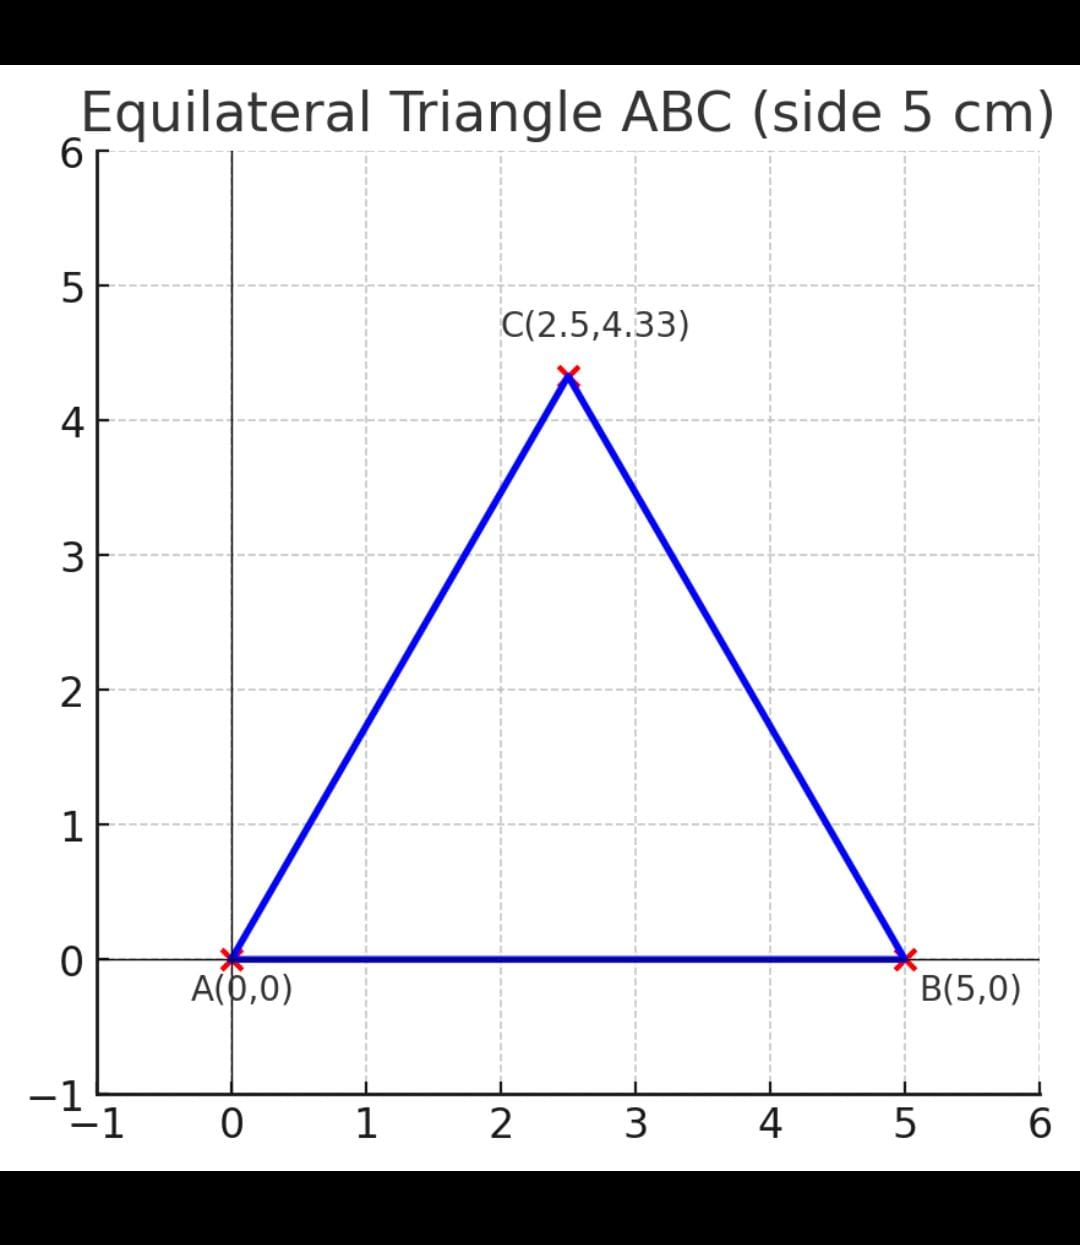
\includegraphics[width=0.65\textwidth]{matgeo-3.3.3.jpeg}
    \caption{}
    \label{fig:triangle5cm}
\end{figure}
\end{frame}

\end{document}
